%%%%%%%%%%%%%%%%%%%%%%%%%%%%%%%%%%%%%%%%%%%%%%%%%%%%%%%%%%%%%%%%%%%%%%%%
%                                                                      %
%     File: Thesis_Kinematics_Dynamics                                 %
%     Tex Master: Thesis.tex                                           %
%                                                                      %
%     Author: Francisco Castro                                         %
%     Last modified :  16 Jan 2024                                     %
%                                                                      %
%%%%%%%%%%%%%%%%%%%%%%%%%%%%%%%%%%%%%%%%%%%%%%%%%%%%%%%%%%%%%%%%%%%%%%%%

\chapter{State of the art}
\label{chapter:stateArt}

This chapter presents a comprehensive literature review on the topics that are adressed in this thesis. Section \ref{section:pathPlanningAlgorithms} outlines a review on the most common world modelling and path planning methods applied to rough terrain. Section \ref{section:ocpRoughTerrain} points to some optimal control applications on rough terrain, that are somewhat close to what is achieved in this thesis.

\section{Path planning algorithms}
\label{section:pathPlanningAlgorithms}

In this section, a review on the generation of path methods for mobile robots is presented. An introductory review to rough terrain path planning is presented in \cite{Spero2002Path}. Moreover, a review on the modelling of maps for optimal path planning is also presented, based on the review of \cite{chapter45handbookrobotics}.

\subsection{World modelling}
\label{subsection:worldModelling}

World modelling falls into one of the following categories (figure \ref{fig:worldsMaps}): indoor and structured environments, natural terrains or dynamic environments. In this thesis, one is interested in performing a metrical evaluation of a mars-like environment with the abscence of dynamic obstacles, so a brief review of models for natural terrains is presented.

\begin{figure}[h]
\centering
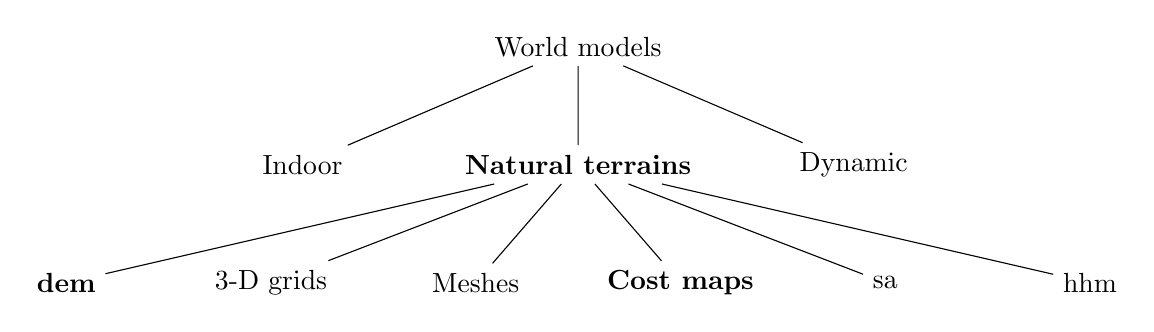
\begin{tikzpicture}[level 1/.style={sibling distance=35mm},
         			level 2/.style={sibling distance=26mm}]
  \node {World models}
    child {node {Indoor}}
    child {node {\textbf{Natural terrains}}
      child {node {\textbf{\acrshort{dem}}}}
      child {node {3-D grids}}
      child {node {Meshes}}
      child {node {\textbf{Cost maps}}}
      child {node {\acrshort{sa}}}
      child {node {\acrshort{hhm}}}}
    child {node {Dynamic}};
\end{tikzpicture}
\caption{World models and map types}
\label{fig:worldsMaps}
\end{figure}

Elevation grids or \tb{digital elevation maps} (\acrshort{dem}) are geometric models which store the elevation $\z$ of a discrete location $(\x_i, \y_j)$. Elevation grids are generated due to sensor data. This retrieval of data may be aerial or on the ground. In case of aerial retrieved data, a regularly sampled grid is typically the end result, due to uniform sensor data. If data is retrieved from the ground, the quality of the data depends on the incidence angle and the distance of the sensor to the location $(\x_i, \y_j)$, which typically yields a variable-sized grid. In the work of \citet{fankhauser2014robot}, a robot-centric, online updated elevation map is estimated, where each cell stores a height estimate $\hat{\z}$ and a variance $\hat{\sigma}_z^2$. From a wheeled, mobile planetary exploration point of view, in \cite{Correal2011} a robot-centered \acrshort{dem} is built from a 3D point cloud, which was generated by a pair of stereo cameras. Aerial data \cite{Smith2001} is also used to deliver an \ti{a-priori} global grid of the target environment, with an accuracy that can be improved by a ground, robot-centered mapping system \cite{Jayasekara2012, Correal2011}.  Additionally, information on how to tackle issues such as sensor resolution, uncertainty and terrain occlusion can be found in \cite{chapter45handbookrobotics}.

\tb{3-D grids and point sets} extend the previous approach to a \acrshort{3d} representation. Typically, this approach handle large sets of points where free or occupied areas can't be defined directly. Octotrees are a solution to this problem. Then, the Octomap approach \cite{Jayasekara2012} uses octotrees to support compact memory representation, multiresolution queries and probabilistic occupancy estimates. A great advantage is that it is possible to model areas which are occluded by vegetation and assign occupancy costs to them.

\tb{Meshes} present an improvement to \acrlong{dem} and 3-D grids. It's a compact representation and presents continuity over the surface. However, this method requires simplifications techniques to lower computational costs and presents some difficulty on defining complex environments as a continuous surface, such as vegetation. Therefore, precise data is needed so that discontinuities are detected.

\tb{Cost maps} are a feasible way to model traversability costs of a rough, uneven terrain and offer a safe and well-known approach to guidance systems on such kind of environments. \tb{Cost maps} may be updated \ti{in-situ} or generated \ti{prior} to placement with overhead imagery. Usually, the computation of costs takes into account the robot kinematics \cite{Amorim2014} and dynamics \cite{Yokokohji2007}, as well as terrain inclination. The definition of an explicit cost function is arbitrary, although the robot's limitations are a factor to include. At the end, the obtained traversability map can be combined with a minimum-cost planner \cite{Amorim2014, Ishigami2007PathPlanning}, in order to output optimal paths into a control system. In the work of \citet{Amorim2014}, a traversability cost is generated at each point by minimizing the height of a mobile robot at each location $(\x_i, \y_j)$. That minimization is carried out by fixing the center of mass of the robot at $(\x_i, \y_j)$, and then the mobile robot is rotated until the lowest admissable height is achieved. In the work of \citet{Ishigami2007PathPlanning}, a criteria function for the \tb{Dijkstra's} algorithm is described, by assigning to each cell a cost, that takes into account the terrain roughness around that cell, the distance to goal and terrain inclination. In \cite{Ventura2015}, a \tb{cost map} is created for an occupancy grid, by making obstacle space impossible to traverse and close to obstacle cells progressively less costly to traverse until a safety distance is reached.

\tb{Semantic attributes} (\tb{\acrshort{sa}}) provide information about the type of terrain and objects found. This representation is called a \ti{high-level} one, in the sense that it groups data into broader classes of data, such as traversable or occupied regions, terrain type or vegetation. On the other hand, the previous approaches are defined as \ti{low-level}. Terrain classification methods \cite{Brooks2012self} are used to determine the type of terrain and landmark extraction is useful to detect saliencies in the environment.

Finally, \tb{Heterogeneous and hierarchical models} (\tb{\acrshort{hhm}}) offer hybrid maps which combine metric and feature maps. In \cite{Fankhauser2016GridMapLibrary}, a \verb!C++! library with Robot Operating System (\acrshort{ros}) and OpenCV interfaces is described. It manages a multi-layer map for rough terrain navigation. It is designed to store data such as elevation, traversability and surface normals.

\subsection{Path planning}
\label{subsection:pathPlanning} 

In rough terrain path planning literature, \textbf{artificial potential fields}, \textbf{optimal path planners} and \textbf{graph-search} algorithms arise as the main choices.

\begin{figure}[h]
\centering
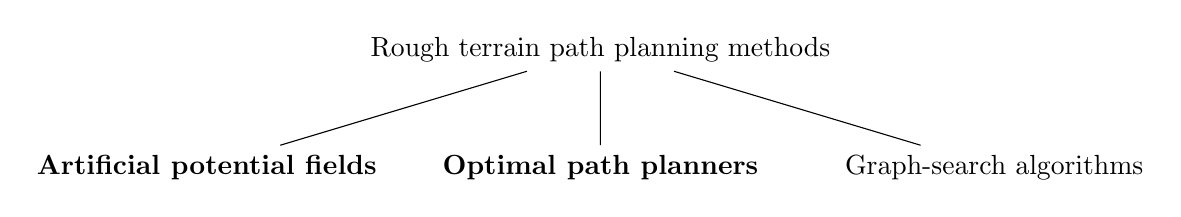
\begin{tikzpicture}[level 1/.style={sibling distance=50mm}]
  \node {Rough terrain path planning methods}
    child {node {\textbf{Artificial potential fields}}}
    child {node {\textbf{Optimal path planners}}}
    child {node {Graph-search algorithms}};
\end{tikzpicture}
\caption{Families of usual path planning methods on rough terrain.}
\label{fig:pathPlanningMethods}
\end{figure}

In \cite{Ishigami2007PathPlanning}, the \textbf{Dijkstra's} algorithm is chosen due to its guaranteed convergence feature, but also because it allows for the optimization of a multiple-metric cost function. In \cite{Spero2002Path}, a \textbf{RRT} method is developped to apply a kinodynamic path planner to a 3D tessellated model. \cite{sakayori2021energy} builds on top of \cite{Ishigami2007PathPlanning} and delivers a \textbf{Dijkstra's} based path planner that also takes into account the energy consumed by the rover when it moves between two nodes. Then, \cite{howard2007optimal} delivers an \textbf{optimal based} trajectory generation algorithm that aims to output a safe trajectory within a real-time window. This method includes the dynamics model of the rover into the \acrshort{nlp}, compensates against wheel slippage and includes terrain uneveness into the method. 

\textbf{Artificial potential field} methods are also extensively used in rough terrain path planning. In the work of \citet{Amorim2014}, the \textbf{fast marching} method is employed in order to output an optimal path between two points. This method guarantees convergence as there aren't local minimums. On the other hand, the goal point matches with the global minimum of the potential field, that helps generating the requested path from any given starting point. In \cite{garridoFMrovers2016}, more evidence is collected that ensures this method is capable of avoiding highly untraversable areas. Finally, a comparison between \textbf{RRT} and the \textbf{fast marching} method is laid out in \cite{garrido2009smooth}, where it is shown that the fast marching method outperforms RRT, not only on the path generation time, but also due to the fact that the fast marching method outputs a shorter path.

In this thesis, it was decided to come with a path planning method on top of the work of \citet{Amorim2014}, as this implementation guarantees completeness, safeness and feasibility for a real-time reference path update, within a real-time control algorithm.

\section{\texorpdfstring{\acrlong{ocp}}{Optimal Control Problem} applications to rough terrain}
\label{section:ocpRoughTerrain}

In this section, some \textbf{\acrlong{ocp}} applications are presented. In \cite{IagnemmaDubowsy2004} a comparison between a velocity-controlled and a rough terrain control system is presented. In this paper, an optimization is performed in order to achieve the desired wheel torques, that safeguard against terrain failure or accounts for power consumption depending on the terrain uneveness. The \textbf{wheel-terrain contact angles} are also estimated in order to include terrain irregularity into the model. At the end, the rough-terrain control system outperforms in terms of the average recorded slip and generally performs well on highly challenging terrain, because the rough terrain control system accounts for the dynamics of the robot, whereas the velocity-based control system does not. However, the authors only tested the algorithm on longitudinal paths and didn't account for roll effects or change of directions.

With the same spirit, the work of \citet{bussmannPlanetaryRoverImpedanceControl} developped a cartesian impedance control that outputs some desired wrench to be followed. Then, an optimization problem is employed to properly distribute the wheel forces, in order to account for wheel-terrain constraints but also to meet the desired impedance wrench. The cost matrices were also manipulated whether power minimization was of interest or not, as saving power may increase the amount of returned science. The authors tested their implementation on a surface with different frictions, which resembles the fact that on a planetary terrain, the surface may go from rocky to sandy. Generally, the method compensates against slip and tracks the desired wrench, although it can only optimize for one feature at a time.

In \cite{lbnmpcOstafew}, a \textbf{nonlinear model predictive control algorithm} is applied to a skid-steering robot that follows a closed path repeatedly. The kinematics is included in the model, but the dynamics is learned through a \textbf{gaussian process model}. The method achieves good tracking results, although it was not tested against high slopes. On the other hand, the works of \citet{binet2012model} and \citet{yu2022nmpc} present applications of \acrshort{nmpc} to wheeled mobile robots, which are closer to what is intended to achieve in this thesis. In \citet{binet2012model}, a \textbf{cascaded \acrshort{nmpc}} method outputs good tracking under a high-fidelity terramechanics dynamics model. It nicely avoids obstacles, although it was not tested under very irregular terrain. In \citet{yu2022nmpc}, the author proposed an integration of the dynamics model into the \acrshort{nmpc}, although it assumed that the mobile robot operates on a plane when the state of the robot is forward integrated along the \textbf{control horizon}. Moreover, the \textbf{bicycle model} is chosen as the wheel-terrain interaction dynamics and wheel-terrain contact angles are not taken into account as well. In this thesis, one is looking to implement the \textbf{Coulomb friction model} as the wheel-terrain interaction dynamics.

Although \cite{rathod2021model} presents a \acrshort{nmpc} application to a legged robot, it is closer to what it is intended to deliver in this thesis, even if only longitudinal trajectories were fed to the controller. The authors introduced the contact angles into the model and a complete 6-\acrshort{dof}s dynamics. The coulomb friction model was also considered in order to avoid slippage. The main goal of the paper was to show a control method that properly ensures mobility and safety, as the authors tracked the motion of the robot against the \textbf{\acrlong{zmp} margin} and ensured that friction forces stay well inside the \textbf{friction cone}. \texttt{acados} \cite{verschueren2022acados} was used for implementing a fast \acrshort{nmpc} solver, like one aims to do in this thesis.

\textbf{Racing} focused \acrshort{nmpc} formulations \cite{liniger2015optimization, mpc_frenetserret} also provide important insights, as these approaches aim to minimize traversal time and safeguard safety, by encouraging progress along the path within the vehicle limitations. In thesis, a \textbf{virtual speed} state is included inside or outside the model, that aims to maximize fastness. \cite{kloesernmpc} uses a constant virtual speed state outside of the solver to maximize progress along the track. \textbf{Obstacle avoidance} is ensured and real-time specs are met by using \texttt{acados} to implement the well-known \textbf{\acrlong{rti} method} (see subsection \ref{subsection:nmpc}).